%%%%%%%%%%%%%%%%%%%%%%%%%%%%%%%%%%%%%%%%%
% Beamer Presentation
% LaTeX Template
% Version 1.0 (10/11/12)
%
% This template has been downloaded from:
% http://www.LaTeXTemplates.com
%
% License:
% CC BY-NC-SA 3.0 (http://creativecommons.org/licenses/by-nc-sa/3.0/)
%
%%%%%%%%%%%%%%%%%%%%%%%%%%%%%%%%%%%%%%%%%

%----------------------------------------------------------------------------------------
%	PACKAGES AND THEMES
%----------------------------------------------------------------------------------------

\documentclass{beamer}

\mode<presentation> {
\usepackage[utf8]{vietnam}
\newcommand\tab[1][1cm]{\hspace*{#1}}


\newcommand{\matrixFormat}[1]{
	/textbf{/textit{#1}}
}

\newcommand{\vectorFormat}[1]{
	/textbf{#1}
}

\newcommand{\scalaFormat}[1]{
	/textit{#1}
}

\graphicspath{ {images/} }
% The Beamer class comes with a number of default slide themes
% which change the colors and layouts of slides. Below this is a list
% of all the themes, uncomment each in turn to see what they look like.

%\usetheme{default}
%\usetheme{AnnArbor}
%\usetheme{Antibes}
%\usetheme{Bergen}
%\usetheme{Berkeley}
%\usetheme{Berlin}
%\usetheme{Boadilla}
%\usetheme{CambridgeUS}
%\usetheme{Copenhagen}
%\usetheme{Darmstadt}
%\usetheme{Dresden}
%\usetheme{Frankfurt}
%\usetheme{Goettingen}
%\usetheme{Hannover}
%\usetheme{Ilmenau}
%\usetheme{JuanLesPins}
%\usetheme{Luebeck}
\usetheme{Madrid}
%\usetheme{Malmoe}
%\usetheme{Marburg}
%\usetheme{Montpellier}
%\usetheme{PaloAlto}
%\usetheme{Pittsburgh}
%\usetheme{Rochester}
%\usetheme{Singapore}
%\usetheme{Szeged}
%\usetheme{Warsaw}

% As well as themes, the Beamer class has a number of color themes
% for any slide theme. Uncomment each of these in turn to see how it
% changes the colors of your current slide theme.

%\usecolortheme{albatross}
%\usecolortheme{beaver}
%\usecolortheme{beetle}
%\usecolortheme{crane}
%\usecolortheme{dolphin}
%\usecolortheme{dove}
%\usecolortheme{fly}
%\usecolortheme{lily}
%\usecolortheme{orchid}
%\usecolortheme{rose}
%\usecolortheme{seagull}
%\usecolortheme{seahorse}
%\usecolortheme{whale}
%\usecolortheme{wolverine}

%\setbeamertemplate{footline} % To remove the footer line in all slides uncomment this line
%\setbeamertemplate{footline}[page number] % To replace the footer line in all slides with a simple slide count uncomment this line

%\setbeamertemplate{navigation symbols}{} % To remove the navigation symbols from the bottom of all slides uncomment this line
}

\usepackage{graphicx} % Allows including images
\usepackage{booktabs} % Allows the use of \toprule, \midrule and \bottomrule in tables
\usepackage{caption}
\usepackage{fancyvrb}
\usepackage{bbm}
\usepackage{wrapfig}
%----------------------------------------------------------------------------------------
%	TITLE PAGE
%----------------------------------------------------------------------------------------

\title[Nhận diện biểu thức toán học viết tay]{Nhận diện biểu thức toán học viết tay bằng phương pháp Watch - Attention - Parse}

\author{Phan Tấn Phúc - Bùi Khánh Ngọc} % Your name
\institute[BKU] % Your institution as it will appear on the bottom of every slide, may be shorthand to save space
{
Ho Chi Minh City University of Technology \\ % Your institution for the title page
\medskip
\textit{\{phantanphuc2512, buikhanhngoc142\}@gmail.com} % Your email address
}
\date{\today} % Date, can be changed to a custom date

\begin{document}

\begin{frame}
\titlepage % Print the title page as the first slide
\end{frame}

\begin{frame}
\frametitle{Overview} % Table of contents slide, comment this block out to remove it
\setcounter{tocdepth}{1}
\tableofcontents % Throughout your presentation, if you choose to use \section{} and \subsection{} commands, these will automatically be printed on this slide as an overview of your presentation
\end{frame}

%----------------------------------------------------------------------------------------
%	PRESENTATION SLIDES
%----------------------------------------------------------------------------------------



\section{Giới thiệu sơ lược}
\subsection{a}
%------------------------------------------------

\begin{frame}
	\frametitle{Giới thiệu Mạng nơron hồi quy (RNN) \footnote{Thuật ngữ tiếng anh: Recurrent Neural Network}}
	{\Huge Giới thiệu Mạng nơron hồi quy (RNN)}
\end{frame}

%------------------------------------------------
\section{Cấu trúc hệ thống}
\subsection{Watcher}

\begin{frame}
	\frametitle{Watcher}
	{\Huge Watcher}
\end{frame}

\begin{frame}
	Watcher bản chất là một hệ thống các lớp convolution tạo thành một mạng Fully Convolutional Network (FCN). Cấu trúc của khối watcher được thể hiện qua sơ đồ sau:\\
	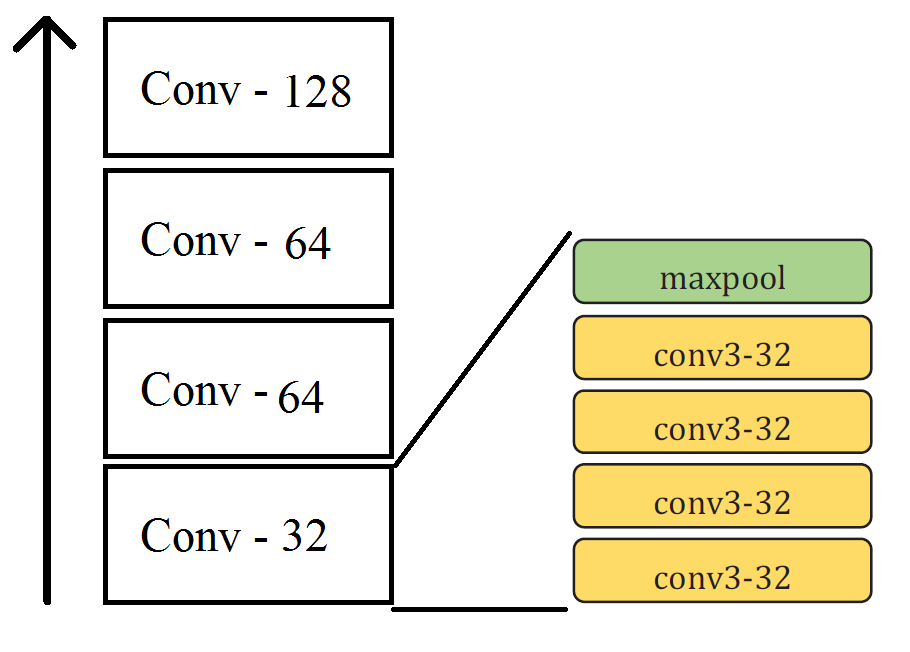
\includegraphics[width=0.9\linewidth]{FCN_Summary.png}
\end{frame}

\begin{frame}
	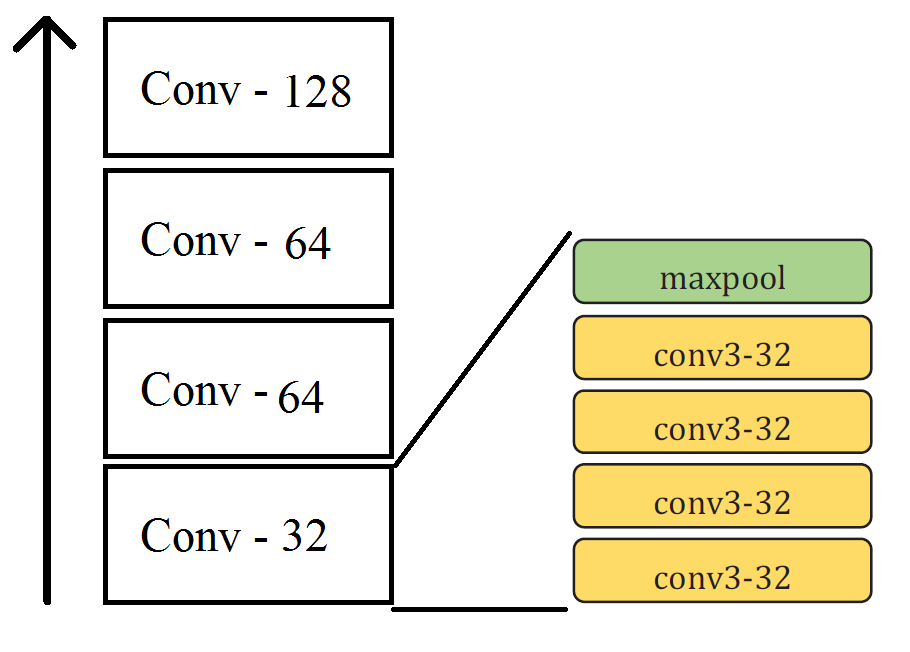
\includegraphics[width=0.5\linewidth]{FCN_Summary.png}\\
	Trong đó, mỗi khối conv được cấu thành bởi 4 lớp convolution liên tiếp và một lớp max-pooling. Các lớp convolution này sử dụng kernel có kích thước $3\times 3$ và sử dụng stride bắng 1 và padding bằng 1. Sau mỗi lớp convolution thì tensor sẽ được đi qua hàm relu. Sau đó, ở cuối mỗi khối Conv là một lớp max-pooling với stride bằng 2 và sử dụng kernel $ 2\times 2$.\\
	Có 4 khối Conv chồng lên nhau có bản chất khá giống nhau (đều là những lớp convolution với kenel $ 3 \times 3$) nhưng với mỗi khối thì có số kernel khác nhau (từ đó thì đầu ra của mỗi layer trong các khối sẽ có số kênh khác nhau - 32, 64 hoặc 128)
\end{frame}
\begin{frame}
	%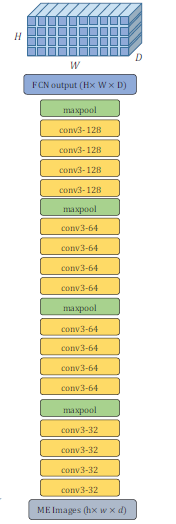
\includegraphics[width=0.25\linewidth]{FCN.png}
	
	\begin{wrapfigure}{l}{0.25\textwidth}
		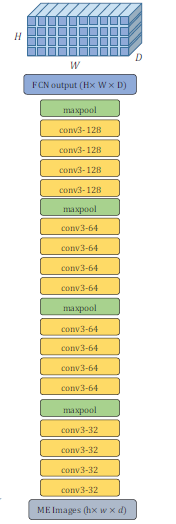
\includegraphics[width=0.7\linewidth]{FCN.png} 
		\caption{Caption1}
		\label{fig:subim1}
	\end{wrapfigure}
	
	
	Hình ảnh bên là mô hình đầy đủ của khối Watcher với một số đặc điểm:
	\begin{itemize}
		\item Mạng nhận dữ liệu đầu vào là khối tensor $ 9 \times w \times h$. Với w, h là kích thước ảnh. 9 kênh của dữ liệu đầu vào bao gồm ảnh 8 hướng của ảnh biểu thức (chiếm 8 kênh) và chính bản thân ảnh đầu vào. Mức xám của ảnh đầu vào là 0 hoặc 1.
		\item Mạng cho dữ liệu đầu ra là một khối tensor $a$ có kích thước $H \times W \times D$.
	\end{itemize}

\end{frame}

%------------------------------------------------
\subsection{Attention}

\begin{frame}
	\frametitle{Attention}
	{\Huge Attentions}
\end{frame}

\begin{frame}
	Trung tâm của khối Attention là một mạng GRU biến thể kết hợp với một số lớp liên kết đầy đủ\footnote{Thuật ngữ tiếng anh: Fully Connected Layer} được cấu trúc đặc biệt theo sơ đồ sau:\\
	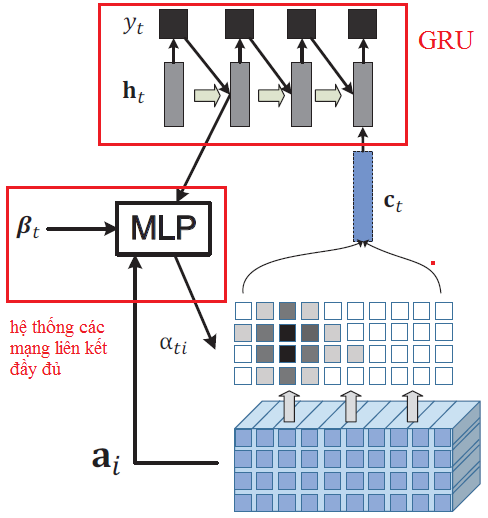
\includegraphics[width=0.5\linewidth]{Attention_img.png} 
\end{frame}

\begin{frame}
	\frametitle{Vector $C_t$ và ma trận $\alpha$}
	Cơ chế Attention là từ trạng thái hiện tại, mạng sẽ sinh ra một "ảnh" $\alpha$, đây là một phân phối xác suất của vị trí của ký tự tiếp theo cần được nhận diện. Ma trận $\alpha$ có kích thước chiều dài và rộng bằng với khối tensor $a$ nhưng chỉ có một kênh, kênh này có các phần tử có giá trị từ $0 - 1.0$ biểu thị xác suất xuất hiện của ký tự tiếp theo cần nhận diện. Do $\alpha$ là một phân phối xác suất, tổng giá trị các phần tử trong $\alpha$ bằng 1.0.\\
	$C_t$ là dữ liệu đầu vào của mạng GRU, $C_t$ được sinh ra theo các bước:
	\begin{itemize}
		\item Nhân từng vector của $a$ (lấy theo chiều sâu) nhân với từng giá trị tương ứng trong $\alpha$, giả sử ta gọi kết quả của phép nhân này là $a'$. Vậy ta sẽ có công thức: $a'_i = a_i \times \alpha_i$
		\item Từ $a'$, ta cộng dồn các vector $a'_i$ để được vector $C_t$. Ta có công thức: $C_t = \sum_i a'_i = \sum_i a_i\alpha_i $
	\end{itemize}
\end{frame}

\begin{frame}
	\frametitle{Khối GRU}
	Như đã được trình bày, GRU là một biến thể của mạng RNN, vì vậy, nó có khả năng sinh ra một chuỗi từ một giá trị đầu vào (one-to-many), điều này phù hợp với bài toán nhận diện biểu thức toán học do ta phải sinh ra một biểu thức toán học gồm nhiều ký tự từ một hình ảnh.\\
	Các cổng của GRU được hoạt động theo công thức:
	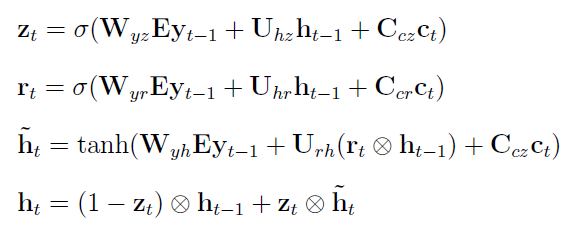
\includegraphics[width=0.7\linewidth]{GRU.png} \\
	Trong đó, $h$ là hidden state của GRU, $y$ là giá ký hiệu đã dự đoán và chỉ số dưới $t$ chỉ vòng lặp GRU thứ $t$.
\end{frame}

\begin{frame}
	\frametitle{Dự đoán ký tự}
	Từ giá trị $h_t$ ở trên, để dự đoán ký tự, ta theo công thức:\\
	$p(y_t|x,y_{t-1}) = \sigma(W_o(Ey_{t-1}+W_hh_t+W_cc_t))$\\
	Trong đó: \\
	$\sigma$ là hàm sigmoid.
\end{frame}

\begin{frame}
	\frametitle{Hệ thống các mạng liên kết đầy đủ}
	Hệ thống này góp phần dự đoán vị trí của ký tự cần dự đoán tiếp theo (cụ thể là tạo ra ma trận $\alpha$), từ đó góp phần sinh vector $c_t$. Việc tạo ma trận $\alpha$ được sinh theo công thức:\\
	\begin{itemize}
		\item $e_{ti} = \nu_a^Ttanh(W_ah_{t-1} + U_aa_i)$: Ở đây, ta lấy giá trị $h_t$ đã được tính ở khối GRU cộng với vector $a_i$, kết quả sẽ được đi qua hàm $tanh$ và tiếp tục đi qua một lớp liên kết đẩy đủ nữa để thu được giá trị $e_{ti}$ tương ứng. Ma trận $e_t$ sẽ có kích thước chiều dài và rộng bằng kích thước của $a$ và chiều sâu bằng 1.\\
		\item $\alpha_{ti} = \frac{e^e_{ti}}{\sum_k e^e_{tk}}$: Sau khi tính được ma trận $e_t$, ta cho $e_t$ đi qua một hàm softmax để cuối cùng thu được một phân phối xác suất, kết quả này chính là ma trận $\alpha$\\
	\end{itemize}
\end{frame}

\begin{frame}
	\frametitle{Coverage}
	Tuy nhiên, nếu chỉ sử dụng mạng với cấu trúc nêu trên, thì việc huấn luyện mạng để sinh ra alpha sẽ gặp khá nhiều khó khăn và từ đó dẫn đến một ký hiệu có thể bị tập trung nhiều lần. Từ đó, tác giả đã đưa vào một nhân tố gọi là Coverage, nhân tố này giúp mạng nắm được các trạng thái tập trung trước đó và điều chỉnh vị trí tập trung tốt hơn.\\
	Nguyên lý hoạt động của nhân tố này là ta sẽ phải cộng dồn các ma trận $\alpha$ lại được ma trận $\beta$, ma trận $\beta$ này sẽ góp phần sinh ra $\alpha$ kế tiếp thông qua việc can thiệp vào công thức:  $e_{ti} = \nu_a^Ttanh(W_ah_{t-1} + U_aa_i)$. Cụ thể:\\
	\begin{itemize}
		\item $\beta_t = \sum_l^{t-1}\alpha_{l}$: Cộng dồn các ma trận $\alpha$.
		\item $F = Q * \beta_t$: trong đó, * là phép convolution, ở đây, ta sẽ cho $\beta_t$ đi qua một lớp convolution, ta sẽ thu được một tensor (thường có cùng kích thước với $a$).
		\item $e_{ti} = \nu_a^Ttanh(W_ah_{t-1} + U_aa_i + U_ff_i)$: Ta tính tỏng các thành đã có lại như đã giải thích ở trên và thêm $U_ff_i$, kết quả sẽ đi qua hàm tanh và tiếp tục đi qua một lớp liên kết đầy đủ $\nu_a^T$
	\end{itemize}
\end{frame}

\begin{frame}
	\frametitle{References}
	Một số link tham khảo:
	Karpathy github:
	https://gist.github.com/karpathy/d4dee566867f8291f086\\
	LSTM - GRU:
	http://colah.github.io/posts/2015-08-Understanding-LSTMs/
\end{frame}


%------------------------------------------------

\begin{frame}
\Huge{\centering{The End}}
\end{frame}

%----------------------------------------------------------------------------------------

\end{document}